\begin{figure}[htbp]
    \centering
    \begin{subfigure}{0.32\textwidth}
        \centering
        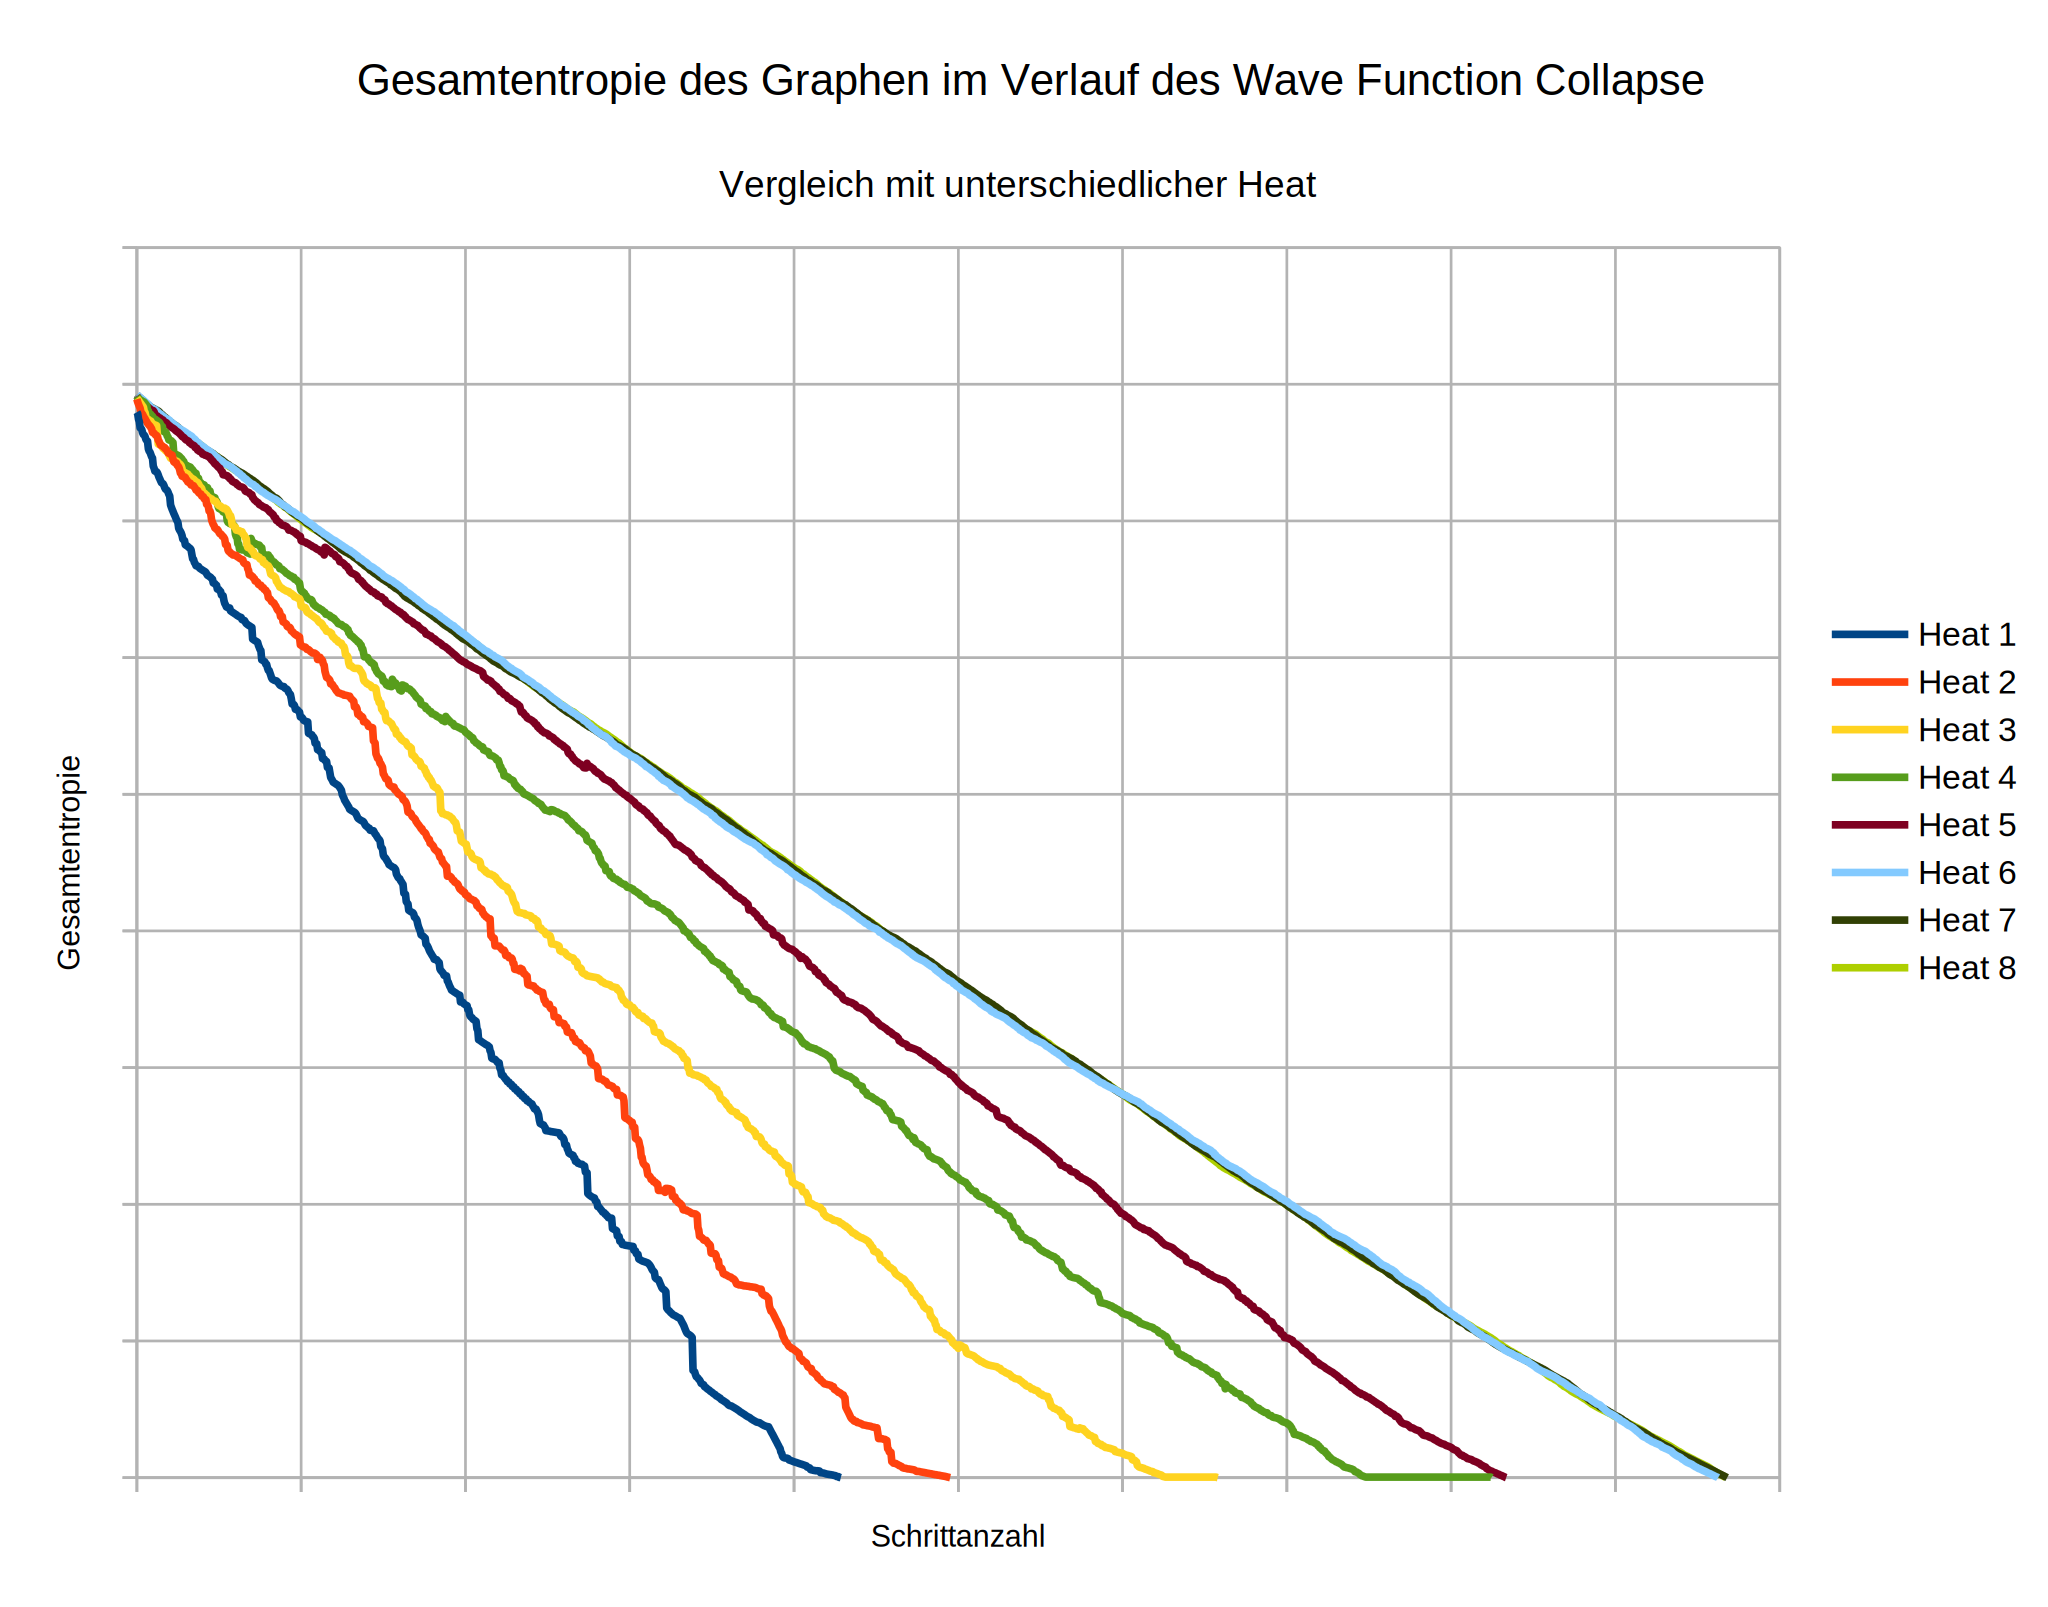
\includegraphics[width=\linewidth]{data/extract_wrapping/1.png}
        \caption{}
    \end{subfigure}\hfill
    \begin{subfigure}{0.32\textwidth}
        \centering
        \includegraphics[width=\linewidth]{data/extract_wrapping/2.png}
        \caption{}
    \end{subfigure}
    \begin{subfigure}{0.32\textwidth}
        \centering
        \includegraphics[width=\linewidth]{data/extract_wrapping/3.png}
        \caption{}
    \end{subfigure}\hfill
    \caption{
        Extrahierung mit N = 2 und vertikalem Wrapping
        \\(a) Das Beispiel ist 4x3 Pixel groß; das erste Umfeld beginnt bei Pixel (0,0)
        \\(b) Umfeld 2 beginnt bei (0,1), die obere Hälfte ist die untere Hälfte von U1
        \\(c) Die untere Hälfte von U3 springt zurück in die erste Zeile
    }
    \label{fig:extract_wrapping}
\end{figure}